\chapter{Discrepancy Theory and Low-Discrepancy Sequences}
\label{chapter2}

% ------------------------------------------------------------------------------
\section{Measuring Uniformity: Discrepancy}
% ------------------------------------------------------------------------------

One of the cornerstones of \ac{qmc} theory is the concept of \emph{discrepancy},
which quantifies how uniformly a finite point set samples the $s$-dimensional
unit cube $[0,1]^s$. While uniform distribution modulo one describes the
asymptotic behavior of infinite sequences, discrepancy provides a finite-sample
measure of deviation from perfect uniformity. Low-discrepancy sequences are the
foundation of \ac{qmc} methods because they minimize this deviation and thus
yield more accurate numerical integration.

This section introduces formal definitions, geometric intuition and empirical
insights into discrepancy measures. It lays the theoretical groundwork for
understanding how the structure of point sets affects \ac{qmc} integration
performance.

% ------------------------------------------------------------------------------
\subsection{Definition of Discrepancy and Star Discrepancy}
% ------------------------------------------------------------------------------

First, we define the more general \emph{extreme discrepancy}:

\begin{definition}[Extreme Discrepancy] \ \\
Let $\mathcal{P}\subset [0,1)^s$, with $|\mathcal{P}| = N$, being a finite point
set. Then the extreme discrepancy $D_N(\mathcal{P})$ is defined as
\begin{equation*}
    D_N(\mathcal{P}) = \sup\limits_{\substack{\boldsymbol{a,b} \in [0,1]^s \\ \boldsymbol{a} \leq \boldsymbol{b}}} \bigg| \frac{A([\boldsymbol{a},\boldsymbol{b}) , \mathcal{P}, N)}{N} - \lambda_s([\boldsymbol{a},\boldsymbol{b})] \bigg|.
\end{equation*}
Hereby $A([\boldsymbol{a},\boldsymbol{b}), \mathcal{P}, N)$ denotes the number
of points in $\mathcal{P}$ that fall into the box
$[\boldsymbol{a},\boldsymbol{b})$, and
$\lambda_s([\boldsymbol{a},\boldsymbol{b})]$ is the Lebesgue measure of that
box, given by $\prod_{i=1}^{s} (b_i - a_i)$.
\end{definition}

In practice, a common and slightly more tractable variant is the \emph{star
discrepancy}, which restricts the test boxes to be anchored at the origin.

\begin{definition}[Star Discrepancy] \ \\
Let $\mathcal{P}\subset [0,1)^s$, with $|\mathcal{P}| = N$, being a finite point
set. Then the star discrepancy $D_N^*$ is defined as
\begin{equation*}
    D_N^*(\mathcal{P}) = \sup\limits_{\boldsymbol{t} \in [0,1]^s} \bigg| \frac{A([\boldsymbol{0},\boldsymbol{t}), \mathcal{P}, N)}{N} - \lambda_s([\boldsymbol{0},\boldsymbol{t})] \bigg|.
\end{equation*}
\end{definition}

This form is used in the Koksma--Hlawka inequality and serves as a central
measure in \ac{qmc} analysis. Note that both discrepancy definitions are
deterministic and depend solely on the point configuration.

\begin{remark}
A low star discrepancy implies that the empirical distribution of the points
approximates the uniform distribution well over all axis-aligned subrectangles
anchored at the origin.
\end{remark}

% ------------------------------------------------------------------------------
\subsection{Geometric Interpretation and Examples}
% ------------------------------------------------------------------------------

To build geometric intuition, consider the 1-dimensional case. Given $N$ sample
points $x_0, \dots, x_{N-1} \in [0,1)$, we can visualize discrepancy as the
maximum vertical deviation between the empirical distribution function
\begin{equation*}
F_N(t) := \frac{1}{N} \sum_{n=0}^{N-1} \chi_{[0,t)}(x_n)
\end{equation*}
and the uniform cumulative distribution function $F(t) = t$. The discrepancy
corresponds to the largest gap between $F_N(t)$ and $F(t)$.

In higher dimensions, the idea generalizes: the star discrepancy measures the
maximal difference in the number of points falling into an axis-aligned box
$[\boldsymbol{0}, \boldsymbol{t})$ versus the volume of that box. Intuitively,
it quantifies whether the point set "overpopulates" or "underpopulates" certain
regions.

\begin{figure}[H]
\centering
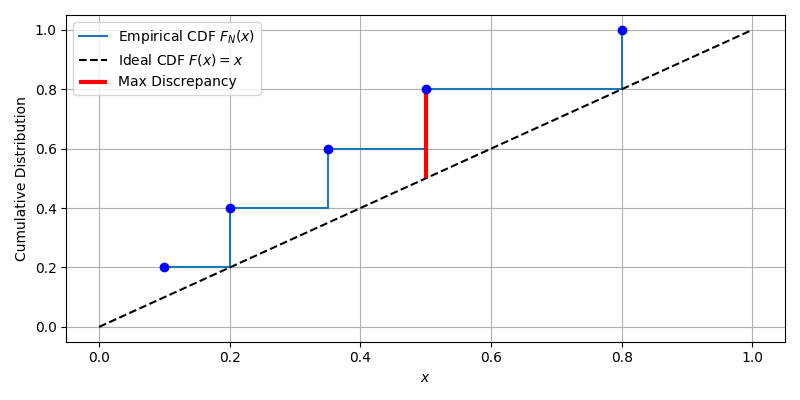
\includegraphics[scale=.67]{Figures/discrepancy1d.png}
\caption{Visualization of 1D discrepancy: the maximum vertical distance between the empirical CDF $F_N(t)$ and the uniform CDF $F(t) = t$.}
\label{fig:discrepancy-1d}
\end{figure}

\begin{example}
Let $x_n = \frac{n}{N}$ for $n = 0, \dots, N-1$. Then $F_N(t)$ is a
piecewise constant staircase function, and the discrepancy can be shown to be
$\mathcal{O}(1/N)$. This is an optimal rate in 1D.
\end{example}

\begin{remark}
Discrepancy provides a worst-case error metric over all subintervals. Thus, even
a point set that appears visually well-distributed may have large discrepancy
due to subtle gaps or clustering in certain regions.
\end{remark}

% ------------------------------------------------------------------------------
\subsection{Empirical Observation of Discrepancy in QMC}
% ------------------------------------------------------------------------------

Discrepancy is not just a theoretical construct -- its practical relevance
becomes evident when comparing the behavior of \ac{qmc} sequences with \ac{mc}
samples. In particular, structured point sets like Halton and Sobol sequences
achieve much lower discrepancy than random samples of the same size.

\begin{figure}[H]
\centering
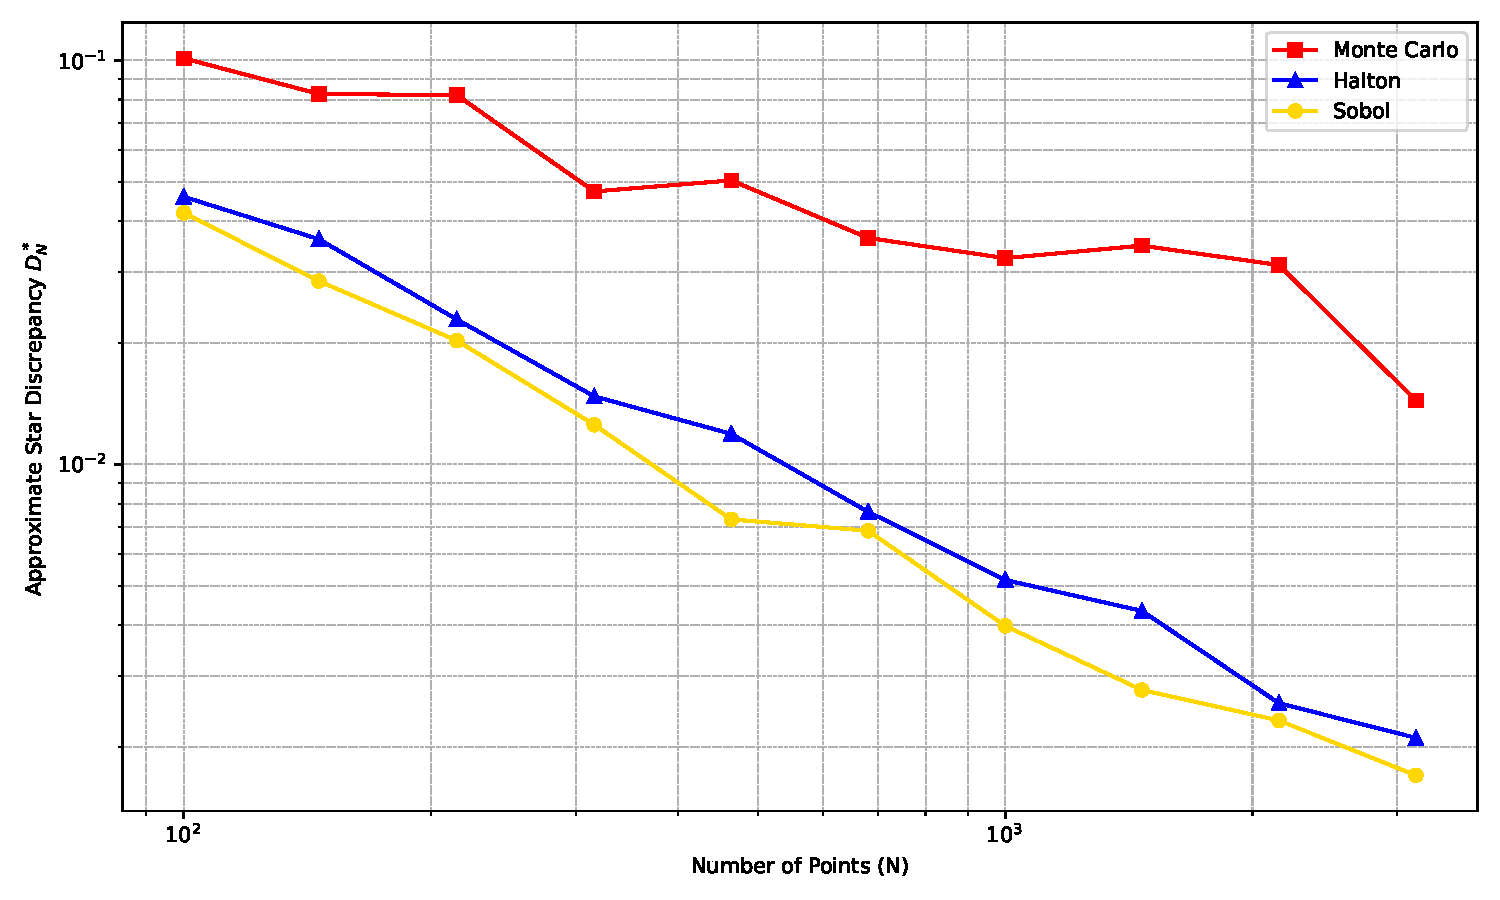
\includegraphics[width=0.9\textwidth]{Figures/qmc_discrepancy_comparison.pdf}
\caption{Comparison of discrepancy growth for Sobol, Halton and random (\ac{mc})
point sets in 2D. Low-discrepancy sequences exhibit significantly slower
discrepancy growth.}
\label{fig:qmc-discrepancy-comparison}
\end{figure}

\begin{remark}
The expected star discrepancy of i.i.d. Monte Carlo samples decreases at the
rate $\mathcal{O}(N^{-1/2})$, whereas for low-discrepancy sequences, provable
upper bounds of order $\mathcal{O}((\log N)^s / N)$ exist.
\cite[Section~2.2]{leobacher2014introduction}
\end{remark}

The next section will introduce specific constructions of low-discrepancy
sequences and analyze their dimensional performance and implementation details.


% ------------------------------------------------------------------------------
\section{Construction of Low-Discrepancy Sequences}
% ------------------------------------------------------------------------------
In this section, we will explore several well-known constructions of
low-discrepancy sequences, focusing on their mathematical foundations and
properties.


% ------------------------------------------------------------------------------
\subsection{The Halton Sequence}
\label{subsec:halton-sequence}
% ------------------------------------------------------------------------------

The Halton sequence is one of the earliest and most widely used constructions of low-discrepancy sequences in arbitrary dimensions. It generalizes the one-dimensional van der Corput sequence to multiple dimensions by using mutually prime bases.

\begin{definition}[Halton Sequence]
Let $b_1, \dots, b_s$ be pairwise coprime integers greater than $1$, typically
chosen as the first $s$ prime numbers. The $n$-th point $\boldsymbol{x}_n \in
[0,1)^s$ of the $s$-dimensional Halton sequence is defined componentwise by
\begin{equation*}
    \boldsymbol{x}_n = \left( \phi_{b_1}(n), \dots, \phi_{b_s}(n) \right),
\end{equation*}
where $\phi_b(n)$ denotes the van der Corput radical-inverse function in base
$b$. The Halton sequence is then given by $\mathcal{S}_{b_1, \dots, b_s} = (x_n)_{n\in \mathbb{N}}$.
\end{definition}

\begin{example}[First Elements of the Halton Sequence in 2D] \ \\
Consider the two-dimensional Halton sequence based on the first two prime bases $b_1 = 2$ and $b_2 = 3$. The first three elements are obtained by computing the radical-inverse values $\phi_{b_1}(n)$ and $\phi_{b_2}(n)$ for $n = 1, 2, 3$:

\begin{itemize}
    \item $n = 1$: $\boldsymbol{x}_1 = \left( \phi_2(1), \phi_3(1) \right) = \left( \tfrac{1}{2}, \tfrac{1}{3} \right)$
    \item $n = 2$: $\boldsymbol{x}_2 = \left( \phi_2(2), \phi_3(2) \right) = \left( \tfrac{1}{4}, \tfrac{2}{3} \right)$
    \item $n = 3$: $\boldsymbol{x}_3 = \left( \phi_2(3), \phi_3(3) \right) = \left( \tfrac{3}{4}, \tfrac{1}{9} \right)$
\end{itemize}

This illustrates how the Halton sequence fills the unit square in a low-discrepancy manner even for small $n$.
\end{example}




The radical-inverse function $\phi_b(n)$ maps an integer $n$ to a real number in $[0,1)$ by reflecting its base-$b$ representation about the decimal point:
\begin{equation*}
    \phi_b(n) = \sum_{k=0}^\infty d_k b^{-k-1}, \quad \text{where } n = \sum_{k=0}^\infty d_k b^k.
\end{equation*}

Intuitively, this construction ensures that each component of the sequence explores the unit interval in a structured, non-redundant way. By combining several one-dimensional van der Corput sequences in different coprime bases, the resulting multi-dimensional point set avoids regular grid-like patterns and achieves asymptotic uniformity.

The Halton sequence has star discrepancy of order
\begin{equation*}
    D_N^*(\{\boldsymbol{x}_0, \dots, \boldsymbol{x}_{N-1}\}) = \mathcal{O}\left( \frac{(\log N)^s}{N} \right),
\end{equation*}
making it a prototypical example of a low-discrepancy sequence. However, for
larger dimensions, correlation effects between the different base components can
lead to degraded uniformity and higher discrepancy. Variants such as scrambling
or leaping are commonly employed to mitigate this issue.

\begin{remark}
The Halton sequence is extensible in $N$ and $s$, making it suitable for
applications that require growing or adaptive point sets. However, its
performance in high dimensions is often inferior to more modern constructions
like the Sobol sequence.
\end{remark}


% ------------------------------------------------------------------------------
  \subsection{The Sobol Sequence}
% ------------------------------------------------------------------------------



% ------------------------------------------------------------------------------
    \subsubsection{Direction Numbers and Gray Code}
% ------------------------------------------------------------------------------



% ------------------------------------------------------------------------------
    \subsubsection{Scrambling Techniques for Sobol}
% ------------------------------------------------------------------------------



% ------------------------------------------------------------------------------
  \subsection{Dimensional Performance and Sequence Comparison}
% ------------------------------------------------------------------------------
